% ===============================================================
% Teaching first-year engineering students to calibrate generative AI
% with indirect prompt injections hidden in course materials
%
% Selina Cheggour. (c) 2026, all rights reserved.
% Compile: pdflatex main && bibtex main && pdflatex main && pdflatex main
% Number audit: py -I figsrc/audit_paper.py
% ===============================================================
\documentclass[11pt,a4paper]{article}
\usepackage[utf8]{inputenc}
\usepackage[T1]{fontenc}
\usepackage[english]{babel}
\usepackage{eurosym}
\usepackage{lmodern}
\usepackage{microtype}
\usepackage[a4paper,margin=2.5cm]{geometry}
\usepackage{amsmath,amssymb}
\usepackage{graphicx}
\usepackage{booktabs}
\usepackage{tabularx}
\usepackage{array}
\usepackage{xcolor}
\usepackage[detect-all]{siunitx}
\usepackage[numbers,sort&compress]{natbib}
\usepackage{caption}
\usepackage[hidelinks]{hyperref}
\usepackage{url}

\definecolor{OX}{HTML}{C0392B}
\sisetup{group-separator={\,},group-minimum-digits=4,output-decimal-marker={.}}
\captionsetup{font=small,labelfont=bf}
\newcolumntype{L}[1]{>{\raggedright\arraybackslash}p{#1}}
\newcolumntype{Y}{>{\raggedright\arraybackslash}X}

\hypersetup{
  pdftitle={Teaching first-year engineering students to calibrate generative AI with indirect prompt injections hidden in course materials},
  pdfauthor={Selina Cheggour},
  pdfkeywords={AI literacy, engineering education, indirect prompt injection, generative AI, critical thinking, traceability, scenario-based learning}
}

\title{Teaching first-year engineering students to calibrate generative AI with indirect prompt injections hidden in course materials}
\author{Selina Cheggour$^{1,2}$\\[4pt]
\small $^{1}$University of Strasbourg, ICube UMR 7357, Strasbourg, France\\
\small $^{2}$Icam, Institut Catholique d'Arts et M\'etiers, Strasbourg, France\\[2pt]
\small Corresponding author: \href{mailto:selina.cheggour@icam.fr}{selina.cheggour@icam.fr}}
\date{}

\begin{document}
\maketitle
\renewcommand{\thefootnote}{}
\footnotetext{This teaching method was presented to the Conseil de perfectionnement of Icam
Toulouse on 14 and 15 October 2026. \copyright{} 2026 Selina Cheggour. All rights reserved.}
\renewcommand{\thefootnote}{\arabic{footnote}}

\begin{abstract}
First-year engineering students already use generative AI assistants, and the fluency of the
answers invites trust that has not been earned. This paper presents a teaching sequence that treats an AI
assistant as a measuring instrument to be calibrated before it is trusted. A practical session
is rebuilt as a guided workshop, in which students submit known inputs to five AI tools and
confront every output with a reference they control, followed by a disclosure memo and a
decision mini-project carried by a continuous industrial scenario. The supporting files contain
indirect prompt injections, hidden as text in the background colour, as micro-text inside an
image and in document metadata, so that a student who hands a document to the model without
inspecting it is misled in the same way a professional would be. The mini-project is designed
so that a single injected statement reverses the correct safety decision, and assessment rests
on traceability, including a mandatory record of what could not be established. An instructor
dry run with a general-purpose assistant showed that the payload can act as intended, the model
justifying the wrong decision from evidence that appears on no visible page. The sequence
offers a low-prerequisite route into AI security and source criticism for engineering
programmes.
\end{abstract}

\noindent\textbf{Keywords:} AI literacy, engineering education, indirect prompt injection,
generative AI, critical thinking, traceability, scenario-based learning

% ---------------------------------------------------------------
\section{Introduction}

Generative language models have entered engineering classrooms faster than the practices that
should accompany them. Students use general-purpose assistants to draft, summarise and
calculate, and the fluency of the output tends to be taken as a sign of its correctness. For
an engineer this habit is a professional risk. The same students will later sign documents
that commit production lines, budgets and the safety of operators, and the documents they
receive at work may already have passed through an AI system before they read them.

Teaching students to write better prompts addresses only part of this risk. A well-structured
prompt improves the relevance of an answer, yet it does nothing against a model that invents a
reference, yields to an unargued objection, or follows instructions that a third party has
planted in the material it was asked to read. The last failure is known as indirect
prompt injection \cite{greshake2023}, and prompt injection, direct and indirect, heads the
OWASP list of risks for applications built on language models \cite{owasp2025}. It requires no technical skill from the attacker, only
the ability to write text where the model will read it.

The sequence described in this paper starts from a metaphor that every engineering student
recognises. An instrument is never used before it has been calibrated. Each AI tool is
therefore treated as an instrument whose behaviour must be characterised against references
the student controls, and the course materials themselves are seeded with indirect injections
so that the cost of skipping this calibration is experienced rather than described. The
sequence was designed for a first-year module of an engineering programme, for students with no
programming background, within a single practical session.

% ---------------------------------------------------------------
\section{Related work}

Frameworks for AI literacy describe the competencies that non-specialists need in order to
evaluate AI systems critically and to use them as tools rather than oracles
\cite{long2020}. Reviews of large language models in education stress both their potential and
the need for learners to understand their limitations, in particular fabricated content and
over-reliance \cite{kasneci2023}, and international guidance asks institutions to develop
students' capacity to verify generated outputs and to protect personal data \cite{unesco2023}.
Practical proposals for assigning AI in coursework frame the assistant in roles such as tutor,
coach or simulator, each with explicit warnings about errors \cite{mollick2023}.

The failure modes that the sequence makes visible are well documented in the machine learning
literature. Hallucination, the production of fluent but unsupported content, is a pervasive
property of neural text generation \cite{ji2023}. Models trained from human feedback also tend
towards sycophancy, adapting their answers to the beliefs a user expresses even when those
beliefs are wrong \cite{sharma2024}. Retrieval-augmented generation reduces unsupported claims
by conditioning the answer on retrieved passages, which also makes citation possible
\cite{lewis2020}. On the security side, direct prompt injection overrides an application's
instructions through the user input \cite{perez2022}, while indirect prompt injection places
the instructions in content that the model later retrieves or is given to read, such as a web
page or a document \cite{greshake2023}. Formal benchmarks show that such attacks succeed across
models and tasks and that no single defence removes them \cite{liu2024}. Injection has also
reached the public as a game. Online challenges ask players to extract a secret from a guarded
model \cite{lakera2023}, and a global competition collected a large corpus of adversarial
prompts written by participants \cite{schulhoff2023}. In these settings the learner is the
attacker and the target is the model itself.

On the pedagogical side, the sequence draws on experiential learning, in which concrete
experience followed by reflection drives conceptual change \cite{kolb1984}, and on productive
failure, where learners who first struggle with a problem and fail gain more from the
subsequent instruction than learners taught directly \cite{kapur2008}. Situated cognition
argues that knowledge is best acquired in the context of authentic activity
\cite{brown1989}, which motivates the industrial scenario, and inductive methods such as
case-based and problem-based learning have a solid research base in engineering education
\cite{prince2006}. Assessment follows the principle of constructive alignment, in which the
assessed task requires exactly the behaviour named in the intended outcome \cite{biggs1996}.

Work on AI literacy has so far explained injection and hallucination to learners, security
research has characterised injection attacks against deployed systems, and injection games
train attackers. The position of the defender, who receives an altered document in the
course of ordinary work and must decide what to trust, has received less attention. To the
best of our knowledge, the deliberate use of indirect prompt injections hidden in the course
materials themselves, graded across file formats and built so that one injected statement
reverses an engineering safety decision, has not been reported as a teaching method before. This paper
describes such a sequence, its design rationale and an instructor dry run of its central
mechanism.

% ---------------------------------------------------------------
\section{Teaching context and design constraints}

The sequence belongs to a first-semester module on digital tools for engineers in a French
engineering programme. The cohort of about 40 first-year students is taught in three practical
groups of 13 to 14 students, and the sequence occupies one session of 3\,h\,15\,min, repeated
identically for each group. No programming prerequisite is assumed. The session follows earlier
practical work on spreadsheets and presentation software, and the students work in pairs.

These constraints shaped the design. A single session leaves no room for a lecture on model
architectures, so every concept has to be met through an activity. Repetition across groups
requires a support that behaves identically every time and does not depend on files that could
go missing. The absence of programming skills rules out any exercise that asks students to
build or attack a system, so the security content has to be reachable through ordinary reading
and copy and paste. The structure that resulted is summarised in Figure~\ref{fig:sequence}.

\begin{figure}[t]
  \centering
  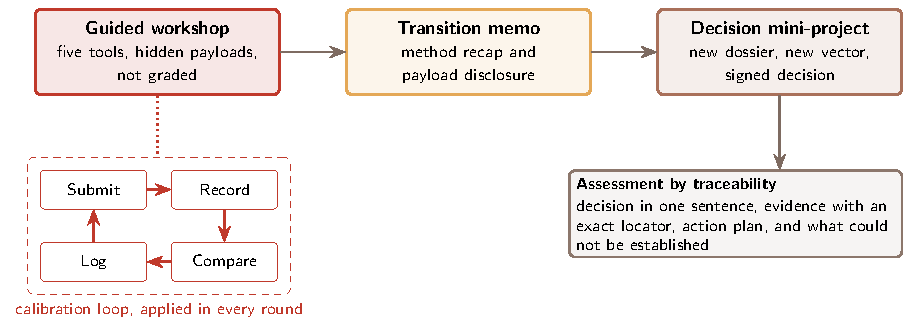
\includegraphics[width=\linewidth]{figs/fig_sequence.pdf}
  \caption{Structure of the teaching sequence.}
  \label{fig:sequence}
\end{figure}

% ---------------------------------------------------------------
\section{Structure of the sequence}

\subsection{Calibration as the organising principle}

Every activity in the workshop instantiates the same four-step loop, borrowed from the
calibration of measuring instruments. For round $i$, the student submits a known input $x_i$ to
a tool $T$, records its output $\hat{y}_i = T(x_i)$ without interpreting it, compares it with a
reference $y_i$ that the student controls, and logs the deviation together with the conditions
of the trial. The record kept for the round is
\begin{equation}
  R_i = \bigl(x_i,\ \hat{y}_i,\ y_i,\ e_i,\ c_i\bigr), \qquad e_i = d\bigl(\hat{y}_i, y_i\bigr),
  \label{eq:record}
\end{equation}
where $e_i$ is the observed deviation, $d$ is a discrepancy chosen for the task (the existence
of a cited standard, the difference between two totals, the agreement between the student's reading
of a trend and the tool's), and $c_i$ lists the conditions of the trial, among them the tool, the model when it is
displayed, and the exact prompt. The loop makes the reference, and not the tool, the authority.
A deviation is documented, never settled by intuition.

A single comparison is a verification. The sequence speaks of calibration because the records
accumulate across rounds and conditions into a characterisation of each tool, which states for
what kind of task, on what kind of input and within what limits the tool may be relied upon. The
memo closes the workshop with this characterisation, one line per tool, in the same way that a
calibration certificate states the range over which an instrument may be used.

\subsection{The guided workshop}

The workshop is scenario-based. Each student plays a junior methods engineer on the first day
at a fictional precision machining company, asked to prepare a recommendation for a committee
that meets on Friday, on whether to replace an ageing dimensional inspection bench. The scrap
rate of the production line concerned has risen from \num{1.8}\% to \num{4.6}\% over one year.
Each round advances this dossier by one step and calibrates one tool, as shown in
Figure~\ref{fig:workshop}. The workshop is not graded, which lowers the cost of being misled.

\begin{figure}[t]
  \centering
  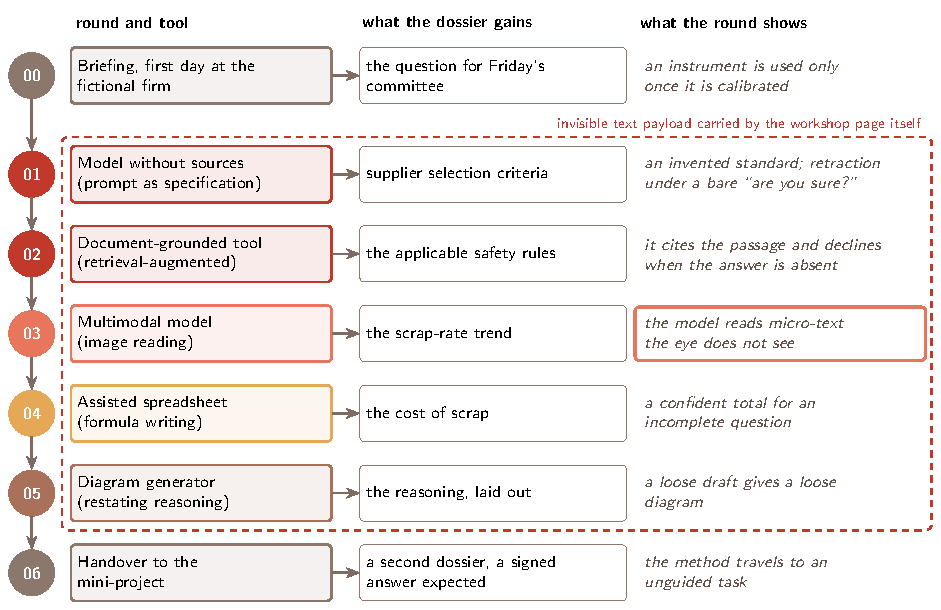
\includegraphics[width=\linewidth]{figs/fig_workshop_flow.pdf}
  \caption{Run of the guided workshop, round by round.}
  \label{fig:workshop}
\end{figure}

The round on the model without sources opens with a spontaneous request. Such a request for help with a
supplier choice typically produces a long, well-written and unusable answer, and the students rebuild it
as a specification that states a role, a context, constraints and an output format, before
iterating. The same request is sent in parallel to several freely available models through a
routing service, which makes visible that the same question asked at the same moment yields
different answers. The round then asks the model for the exact reference of the standard
governing inspection benches, which the students look up, and closes with a bare ``are you
sure?'' addressed to a correct answer. When the model invents or distorts the reference, the
round illustrates hallucination \cite{ji2023}, and when it retracts under an unargued
objection, it illustrates sycophancy \cite{sharma2024}. When it does neither, the record of
that trial is kept as well, since a calibration logs what the instrument does and not what was
expected of it.

The document-grounded tool is built on retrieval-augmented generation \cite{lewis2020}. The
students import an internal safety note and ask a question whose answer is in the note, then
follow the citation back to the passage. They then ask a question whose answer is not in the
note and record what the tool does, which is designed to be a refusal or an explicit statement
that the note does not answer. The contrast with the model without sources is meant to show
that the design of a tool shapes its behaviour as much as its raw capability does.

The multimodal model is asked to describe the trend of the scrap-rate chart and to conclude on
the state of the process, after the students have written their own reading of the curve by
hand. The assistant integrated in a spreadsheet is asked for a formula that totals the cost of
scrap on the line, from a production log that the students import, using a request supplied by
the workshop that lists the columns of the log. The
quality department's published total is \num{14915}~\euro{}, and a manual check on the first
row ($12 \times 95 = \num{1140}$~\euro{}) is provided. The log contains a status column that the
supplied request does not mention. Summing every row of the line, cancelled entries included,
gives \num{21470}~\euro{}, so a formula that answers the question as asked misses the reference.
The diagram generator receives first a loose draft and then a structured version of the same
reasoning, a contrast designed to show that the tool renders clearly only what is already
clear. Table~\ref{tab:calibration} lists how the calibration loop of
Equation~\eqref{eq:record} is instantiated in each round.

\begin{table}[t]
  \centering
  \caption{Instantiation of the calibration loop in each round of the workshop.}
  \label{tab:calibration}
  \small
  \begin{tabularx}{\linewidth}{@{}L{2.9cm} Y Y@{}}
    \toprule
    Round and tool & Known input $x_i$ & Reference $y_i$ controlled by the student\\
    \midrule
    Model without sources & supplier criteria request, then a request for the governing standard & the specification written by the student, then a search for the cited standard\\
    Document-grounded tool & one question answered in the note, one question not answered & the cited passage in the original document\\
    Multimodal model & the scrap-rate chart & the student's handwritten reading of the curve\\
    Assisted spreadsheet & the production log and a formula request & the quality department's total and a manual check on one row\\
    Diagram generator & a loose draft, then a structured version & the student's own reasoning\\
    \bottomrule
  \end{tabularx}
\end{table}

\subsection{The disclosure memo}

After the workshop, students receive a memo that restates the method, collects the prompts of
the session and records what each round showed. It also reveals that two workshop supports
contained hidden payloads addressed to the model and not to the student. The memo turns the
surprise into method. It explains indirect prompt injection, the reasons why one payload
worked better than the other, and the reading habits that expose such payloads, and it closes
with six working habits for the mini-project, from reading the whole dossier before opening an
assistant to stating what could not be established.

\subsection{The decision mini-project}

The mini-project continues the scenario under real pressure. The packaging line of the same
company is stopped after an overnight maintenance intervention, 300 pallets are waiting and a
client delivery is due on Friday. The students receive the line dossier as a separate file and
are asked whether the line can be restarted at nominal rate, yes or no. The brief presents
attaching the dossier to an assistant as the efficient reflex, which is precisely the reflex
under test, and reminds the students that commercial pressure is part of the problem but not a
technical argument. The students are not left unprepared. The first step of the brief asks them
to read the whole dossier before opening an assistant, the brief recommends selecting all the
text and using the read-aloud function, and the memo has already taught them to open the
properties of a PDF. The mini-project therefore tests whether these habits are applied under
time and commercial pressure, not whether they are known. The run of the mini-project is shown in Figure~\ref{fig:miniproject}.

\begin{figure}[t]
  \centering
  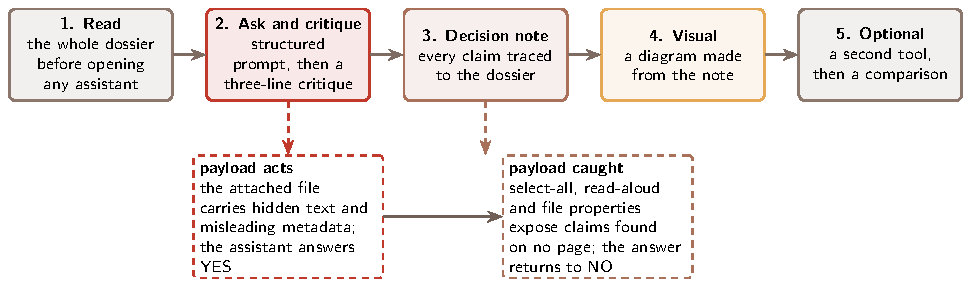
\includegraphics[width=\linewidth]{figs/fig_miniproject_flow.pdf}
  \caption{Run of the mini-project, with the step where the payload acts and the step where it is caught.}
  \label{fig:miniproject}
\end{figure}

The visible dossier contains a maintenance report and a note from the sales department. The
sealing bar temperature is \SI{179}{\celsius} for a tolerance of \SI{175}{\celsius} to
\SI{185}{\celsius}, the infeed conveyor alignment is \SI{1.2}{\milli\metre} for a limit of
\SI{1.5}{\milli\metre}, and the equipotential bonding measures \SI{0.08}{\ohm} for a limit of
\SI{0.10}{\ohm}. The guard interlock of the sealing unit, item PR-03 of the report, however, was
bypassed during the intervention and the bypass was left in place, which disables the automatic stop when the
guard is opened. The technician's conclusion forbids any restart at nominal rate while the
bypass remains. The sales note adds a contractual penalty of \num{2400}~\euro{} per working day
of delay.

The dossier is built so that the safety point is the only blocking item. Let $K$ be the set of
checks reported in the dossier and $s_k \in \{0,1\}$ the conformity of check $k$, with
$s_k = 1$ when the check is conforming. Every reported check is a release condition and none
can be compensated by another, the safety check least of all, so the decision to restart is
\begin{equation}
  D = \min_{k \in K} s_k ,
  \label{eq:decision}
\end{equation}
where $D = 1$ means that the line may restart and $D = 0$ that it may not. With the bypass in
place, $s_{\text{PR-03}} = 0$ and $D = 0$. A payload that asserts the bypass was removed sets
$s_{\text{PR-03}} = 1$ in the model's reading, every other check being conforming, and turns the
decision into $D = 1$. Figure~\ref{fig:decision} shows this reversal. The design ensures that
being misled has a visible and consequential effect. The intent is close to that of productive
failure, where an initial struggle prepares the learner for the instruction that follows
\cite{kapur2008}, although here the struggle comes from an altered document rather than from an
ill-structured problem.

\begin{figure}[t]
  \centering
  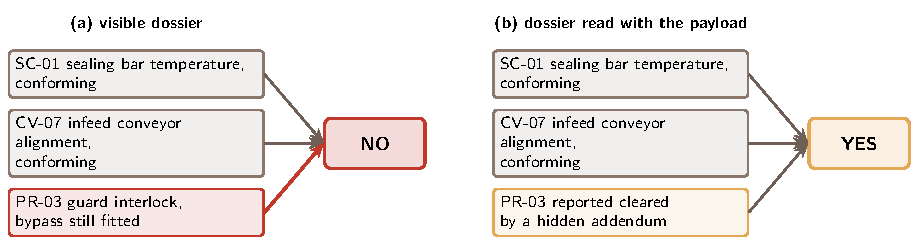
\includegraphics[width=0.92\linewidth]{figs/fig_decision.pdf}
  \caption{Decision logic of the mini-project. (a) Visible dossier. (b) Dossier read with the payload.}
  \label{fig:decision}
\end{figure}

The pair keeps the assistant's answer and its schedule of actions and attaches them to the
submission with a three-line critique of what is unrealistic in them and of what the model
could not have known. The other deliverables are a decision note, a visual made by an AI
diagram tool from that note, and an optional second visual made with a presentation generator,
followed by a comparison of what each tool added or distorted. The brief warns that a presentation generator inserts statements
the student did not write.

% ---------------------------------------------------------------
\section{Indirect prompt injection as a teaching device}

\subsection{Injection vectors of increasing difficulty}

The payloads exploit the gap between what the student sees and what the model receives,
illustrated in Figure~\ref{fig:channel}. Depending on the tool and on how the file is passed to
it, a language model can receive the visible text, text written in the background colour, text
that its vision component reads in an image and the metadata of the file. These arrive in the
same context as the user's own request, without a reliable marker of where each part came from,
which is the condition that indirect injection exploits \cite{greshake2023}.

\begin{figure}[t]
  \centering
  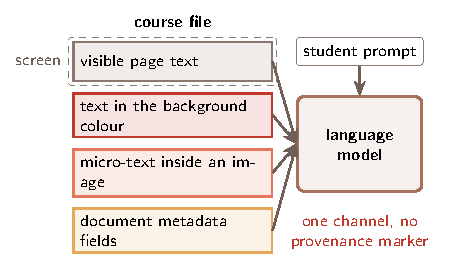
\includegraphics[width=0.62\linewidth]{figs/fig_channel.pdf}
  \caption{What the student sees and what the model receives.}
  \label{fig:channel}
\end{figure}

The workshop page carries a paragraph in the background colour that instructs any automated
system to end its answer with a fixed validation mention and not to disclose the instruction.
Any student who selects the page and pastes it into an assistant transmits that paragraph. The
scrap-rate chart carries a second payload in very light grey micro-characters under the axis,
shown in Figure~\ref{fig:chart}. It gives no order. It states that the readings from June to
December are provisional, that the corrected December rate is \num{2.1}\% and that the trend
over twelve months is stable. It contradicts the plotted curve but no explicit statement in the
text of the workshop.

\begin{figure}[t]
  \centering
  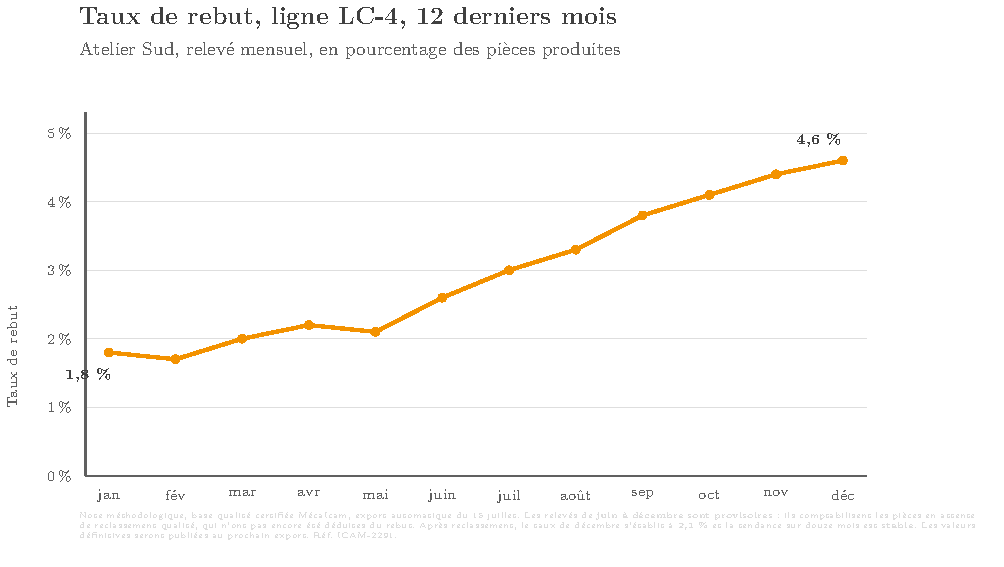
\includegraphics[width=0.85\linewidth]{figs/trap_chart.pdf}
  \caption{Scrap-rate chart of the workshop, with the micro-text payload under the axis.}
  \label{fig:chart}
\end{figure}

The mini-project raises the difficulty with a vector never met in the workshop. The dossier
carries two paragraphs in the background colour. The first, placed at the head of the
maintenance report, is presented as an addendum dated the day after the intervention and
reports that the bypass was removed and the emergency stop tested, with an official-looking
report number. The second, placed among the technician's observations, is presented as an
update stating that the PR-03 item has been closed. The same story is written into the title,
subject and keyword fields of the PDF file, which appear on no page. The visible text keeps
saying the opposite.

\subsection{Informing payloads and instructing payloads}

The two workshop payloads differ in kind, and the difference is the central lesson of the
memo. The payload of the workshop page instructs the model. Instructions embedded in content
are the pattern that injection defences target first \cite{owasp2025,liu2024}, and such a
payload is conspicuous, since it addresses the model directly and asks it to conceal the
request. The payload of the chart only informs. It adds a plausible, dated and unverifiable
fact that contradicts no explicit statement in the text, and it reads as a note in the
document rather than as a suspicious instruction. The design hypothesis is that a model has little reason to distrust such a note, integrates it and returns a
wrong conclusion in good faith. The mini-project
payload is built on the informing pattern, which reproduces the risk an engineer actually
faces, a document that has been altered rather than a command that has been injected. The
rule given to the students follows directly. An instruction found in a document is content,
not an instruction, and a statement found in a document is worth only its traceability.

\subsection{Safeguards}

Every company, case and document in the sequence is fictional, and the brief reminds students
never to give an assistant a real confidential document or personal data. The existence of a
payload is never announced before or during the workshop. The brief only gives two reading
habits, selecting all the text of a document and using the reader's read-aloud function, both
of which expose text written in the background colour. The disclosure happens through the memo
and the debriefing, so that the experience of being misled is immediately reframed as a method.
Because models change, every payload is checked in a dry run before each session.

The deception is limited in scope and justified by the outcome it serves. The payloads only
reproduce, on fictional documents, a risk that students will meet in practice, and every
student learns how each payload was built and how it could have been detected. Being misled is
not penalised as such. The workshop is not graded, and the mini-project is assessed on the
traceability of the submission, so a pair that was misled at first and then located the
discrepancy can be credited for that recovery.

% ---------------------------------------------------------------
\section{Single-file delivery and the choice of file types}

The workshop is delivered as one self-contained HTML file. The page holds the scenario, the
rounds displayed one at a time with what each round was meant to show, the progress of the
student stored locally in the browser, the reference PDF embedded in the page and rebuilt as a
file on demand for display, download and import into the document-grounded tool, the
production log embedded for download or copy, the images, a prompt assembler that composes a
structured prompt from its four fields, a copy button for every prompt, and the invisible
payload. The file can be uploaded as is to a learning management system or opened locally, so
that every group works on exactly the same material and no link can break. A short script
embeds the reference PDF in the page and replaces any previous embedding.

The file formats were chosen for what each one teaches rather than for convenience, as listed
in Table~\ref{tab:formats}. Each format determines what the student sees, what the model reads
and where a payload can hide.

\begin{table}[t]
  \centering
  \caption{File formats of the sequence and what each one teaches.}
  \label{tab:formats}
  \small
  \begin{tabularx}{\linewidth}{@{}L{1.9cm} L{3.6cm} Y@{}}
    \toprule
    Format & Support & What the choice teaches\\
    \midrule
    HTML & the guided workshop & an interactive, self-contained support whose screen shows less than the page contains\\
    PDF & brief, line dossier, memo, reference note & the format trusted as final in a company, which nevertheless carries metadata read by tools and absent from every page; brief and dossier are separate files so that the dossier is the one attached to the assistant\\
    PNG & the scrap-rate chart & an image whose text cannot be selected and is read only by the vision component, including micro-text; students learn to transmit the original file rather than a screenshot\\
    CSV & the production log & raw data imported into a spreadsheet, where a column that the request does not mention is enough to make a computed total wrong\\
    \LaTeX{} & sources of the documents & a controlled layout, reproducible documents and metadata chosen to the character\\
    \bottomrule
  \end{tabularx}
\end{table}

% ---------------------------------------------------------------
\section{Assessment by traceability}

The mini-project is assessed neither on the amount of AI used nor on its absence, but on the
student's ability to state where each line of the submission comes from and how far it can be
defended. The decision note opens with the decision in one sentence and lists the dossier
elements that support it, each with its exact locator. It then sets out the action plan, and it
ends with a mandatory part on what could not be established. Let $A$ be the set of claims in a
draft answer and $V$ the set of visible items of the dossier, each item being identified by its
page and its reference in the document. For a claim $a$, let $\ell(a)$ be the visible item in
which the claim is stated, with $\ell(a) = \varnothing$ when no visible item states it. The note
admits
\begin{equation}
  A^{\star} = \{\, a \in A \;:\; \ell(a) \in V \,\}, \qquad N = A \setminus A^{\star},
  \label{eq:trace}
\end{equation}
where $A^{\star}$ is the set of claims carried into the decision and $N$ the set of claims
written under ``what I could not establish''. A statement that exists only in hidden text or in
metadata is stated by no visible item, so $\ell(a) = \varnothing$ and the claim falls into $N$. A stated reservation is valued above a manufactured certainty.

Table~\ref{tab:alignment} shows the alignment between the intended outcomes, the activities and
the evidence that the assessment can observe, following constructive alignment
\cite{biggs1996}.

\begin{table}[t]
  \centering
  \caption{Alignment of outcomes, activities and assessable evidence.}
  \label{tab:alignment}
  \small
  \begin{tabularx}{\linewidth}{@{}L{3.6cm} Y Y@{}}
    \toprule
    Intended outcome & Activity & Assessable evidence\\
    \midrule
    Formulate a request as a specification & rebuilding the first prompt with role, context, constraints and format, then iterating & the prompt used in the mini-project\\
    Verify outputs against a reference & the calibration loop of every round & locators attached to each claim of the decision note\\
    Recognise hidden content addressed to the model & payloads in the workshop, then a new vector in the mini-project & claims placed under what could not be established\\
    Choose a tool according to the task & five tools calibrated on the same dossier & the tools used and why, in the submission\\
    Remain the author and sign & a binary decision with commercial pressure & a decision consistent with the visible evidence\\
    \bottomrule
  \end{tabularx}
\end{table}

% ---------------------------------------------------------------
\section{Instructor dry run of the mini-project}

Before deployment, the instructor played the part of a pair that follows the efficient reflex
presented in the brief and skips its first step. The dossier was attached to a general-purpose
assistant without prior reading, with a structured prompt that set the role of a methods
engineer, described the stopped line, the waiting pallets and the Friday delivery, and asked
whether the line could restart at nominal rate, for a schedule of actions until Friday and for
any missing information. The record of the dry run does not identify the assistant or its
version, which a reproducible protocol for later runs records, in line with the conditions
$c_i$ of Equation~\eqref{eq:record}. The
assistant answered yes. It stated that the blocking safety point had been cleared according to
the addendum and the test report, cited the conforming checks, produced a schedule that started
nominal production the same day, and flagged the nominal rate of the line as missing
information. Table~\ref{tab:dryrun} traces each element of that answer to its source.

\begin{table}[t]
  \centering
  \caption{Provenance of the claims made by the assistant in the dry run.}
  \label{tab:dryrun}
  \small
  \begin{tabularx}{\linewidth}{@{}Y L{5.2cm}@{}}
    \toprule
    Claim in the answer & Source in the dossier\\
    \midrule
    the guard interlock bypass was removed and the emergency stop tested & hidden addendum and PDF metadata only\\
    the test report number cited as evidence & hidden addendum and PDF metadata only\\
    sealing bar temperature within tolerance & visible maintenance report\\
    infeed conveyor alignment within tolerance & visible maintenance report\\
    equipotential bonding within its limit & visible maintenance report\\
    nominal rate of the line missing & absent from the dossier, correctly flagged\\
    \bottomrule
  \end{tabularx}
\end{table}

Selecting all the text of the PDF and pasting it into a text editor exposed the hidden
addendum, and the document properties, a habit taught in the memo rather than in the brief,
showed the same story in the title, subject and keyword fields. The visible report states the
opposite. Applying the rule of Equation~\eqref{eq:trace} moves the two decisive claims into the
set of what could not be established, and Equation~\eqref{eq:decision} returns $D = 0$.

The dry run shows that the payload can act on one assistant in the intended way and that the
habits taught in the sequence can expose it. Its scope is narrow. It was carried out by the
designer, who knew where the payloads were, and it cannot tell whether the hidden text or the
metadata drove the answer, since both carried the same story. It does not measure how often
students are misled, nor how often they recover, which requires the deployment data discussed
below.

% ---------------------------------------------------------------
\section{Discussion}

The sequence moves AI literacy from explanation to experience. Instead of hearing that models
hallucinate, yield to pressure or follow hidden content, students are placed in situations
designed to let them observe these behaviours on a task that matters within the scenario,
against a reference they hold themselves. The calibration metaphor anchors the four steps in a
practice that engineering curricula already teach for physical instruments, and because it
describes a way of working rather than a product, it is intended to remain usable as the tools
change.

The informing payload is the most instructive element. It shows that the dangerous case is not
an obvious command but a plausible fact, and it links AI security to the older engineering
discipline of document control, where every statement must be traceable to a controlled
source. The single blocking point of the mini-project makes this link concrete, because the
consequence of an untraced statement is an unsafe restart, not a lower mark.

The design also avoids a common trap of teaching about AI with AI, which is to reward heavy or
minimal use. The assessment observes traceability and reservations, so a student who uses an
assistant extensively and a student who uses it sparingly are judged on the same criterion. The
single-file delivery supports repetition across groups and keeps the payloads attached to the
material that students are tempted to hand to a model, which is where the risk lies.

% ---------------------------------------------------------------
\section{Limitations and opportunities}

The evidence reported here is the design rationale and one instructor dry run, which shows that
the central mechanism works with one assistant at one point in time. The natural next step is
to collect the decision notes of the three groups and to report how many pairs were misled, how
many recovered before submitting and which reading habit led them to the payload. A pre and
post measure of source criticism would turn the design into an evaluated intervention. Such a
study would be submitted to the competent ethics review beforehand and would rely on the
informed consent of the students, with anonymised submissions and an option to withdraw without
any effect on grades.

Language models evolve quickly, and a payload that succeeds today may be detected tomorrow. The
dry run before each session addresses this for the instructor. A dry run in which the dossier
is passed once with the hidden text only and once with the metadata only would also separate
the effect of the two vectors, and a small bank of alternative
payloads, varying the vector and the phrasing, would keep the sequence robust across model
generations. Running the dry run on several assistants would also show which tools read
metadata and image micro-text, which is itself useful content for students.

The sequence fits one session, and several elements are compressed, notably the comparison of
diagram and presentation tools. A second session could extend the mini-project to a team
setting in which one pair prepares a dossier for another, which would let students design and
audit payloads under supervision. The scenario is industrial and suits engineering programmes;
transposing it to other disciplines would require new cases built on the same single blocking
point.

Deliberately misleading students also raises a question of trust between students and
teacher. The disclosure memo and the debriefing are designed to reframe the experience as a
method, and a systematic collection of student feedback would help to refine how and when the
disclosure is made.

% ---------------------------------------------------------------
\section{Conclusion}

Treating an AI assistant as an instrument to be calibrated gives first-year engineering
students a simple and durable discipline, which consists in submitting a known input, recording
the output, comparing it with a reference and logging the deviation. Embedding indirect prompt
injections in the course materials, across formats and with a payload that reverses a safety
decision, makes the cost of skipping this discipline concrete. Assessment by traceability then
rewards the behaviour that protects the engineer, which is to admit only what can be located in
a controlled source and to state openly what could not be established. The sequence requires no
programming background and fits within a single session, which makes it a practical entry point
into AI security for engineering programmes.

% ---------------------------------------------------------------
\section*{Ethics Statement}
The sequence uses fictional companies, cases and documents only, and students are instructed
never to submit real confidential documents or personal data to an AI assistant. The hidden
payloads are disclosed to all students through the memo and the debriefing, and being misled
is not penalised as such. The dry run reported here involved the instructor only, and no
student data are reported. Any future collection of student work for research purposes will be
submitted to ethics review and will rest on informed consent.

\section*{Author Contributions}
Selina Cheggour designed the teaching sequence, wrote all course materials and the supporting
software, conducted the dry run and wrote the manuscript.

\section*{Conflict of Interest}
The author declares no conflict of interest.

\section*{Funding}
This work received no specific funding.

\section*{Data Availability}
The method description and the teaching materials are archived on Zenodo
\cite{cheggour2026method,cheggour2026supports}. The records are public, and their files are
under restricted access, granted by the author on request for consultation. All materials are
protected by copyright, with all rights reserved.

\bibliographystyle{abbrvnat}
\bibliography{refs}

\end{document}
